\pSpaceΣτο παρόν κεφάλαιο παρουσιάζεται ένα εγχειρίδιο χρήσης για όλες τις διαθέσιμες σελίδες της εφαρμογής.Χωρίζεται σε τρία μέρη: αρχική σελίδα, εγγραφή/ταυτοποίηση και \e{iPM}.Η κάθε ενότητα περιέχει περιγραφή, οδηγίες και εικόνες που αφορούν την συγκεκριμένη σελίδα η λειτουργία.\\
\pSpaceΕπίσης το τρίτο μέρος που αφορά το \e{iPM}, χωρίζεται σε δύο ενότητες, \e{user} και \e{project}.Το πρώτο εξηγεί τις ενέργειες του χρήστη ως προς το προσωπικό \e{Dashboard, Profile} κλπ, ενώ στο δεύτερο τις ενέργειες που μπορούν να συμβόυν σε ένα έργο.\\
\section{\e{Homepage}}
\pSpaceΗ αρχική σελίδα (βλ. σχ. \ref{fig:homepage}) έχει τον ρόλο ενός \e{landing page}, δηλαδή η σελίδα που θα πρωτοσυναντήσει ο χρήστης όταν αποκτήσει πρόσβαση στην διεύθυνση της εφαρμογής (\e{\url{https://pmthesis.herokuapp.com}}).\\
\pSpaceΧρησιμοποιώντας το μενού που βρίσκεται στον επάνω μέρος της σελίδας, ο χρήστης μπορεί να μετακινηθεί στην ενότητα που τον εδνιαφέρει χωρίς περαιτέρων αλληλεπιδράσεις.\\
\pSpaceΣτην ενότητα \e{Authenticate}, έχει δύο επιλογές για να αποκτήσει πρόσβαση στην εφαρμογή: εγγραφή η σύνδεση με ένα υπαρκτό λογαριασμό.Η πρώτη τον οδηγεί στην διεύθυνση \e{\url{https://pmthesis.herokuapp.com/auth/signup}} ενώ η δεύτερη στην \e{\url{https://pmthesis.herokuapp.com/auth/signin}}.\\
\pSpaceΕπιπλέον στην τελευταία ενότητα, υπάρχει μια φόρμα επικοινωνίας, που έχει ως στόχο την αποστολή ερωτημάτων, προβλημάτων που αφορούν την εφαρμογή.Ακόμη, στο κάτω μέρος της σελίδας υπάρχουν συντομεύσεις για το \e{repository} στο \e{Github}, για την σελίδα του Τμήματος Πληροφορικής Σερρών και μια ακόμη που αφορά οδηγίες χρήσης εφαρμογής.\\
\pagebreak

\begin{figure}[!htb]
\centering
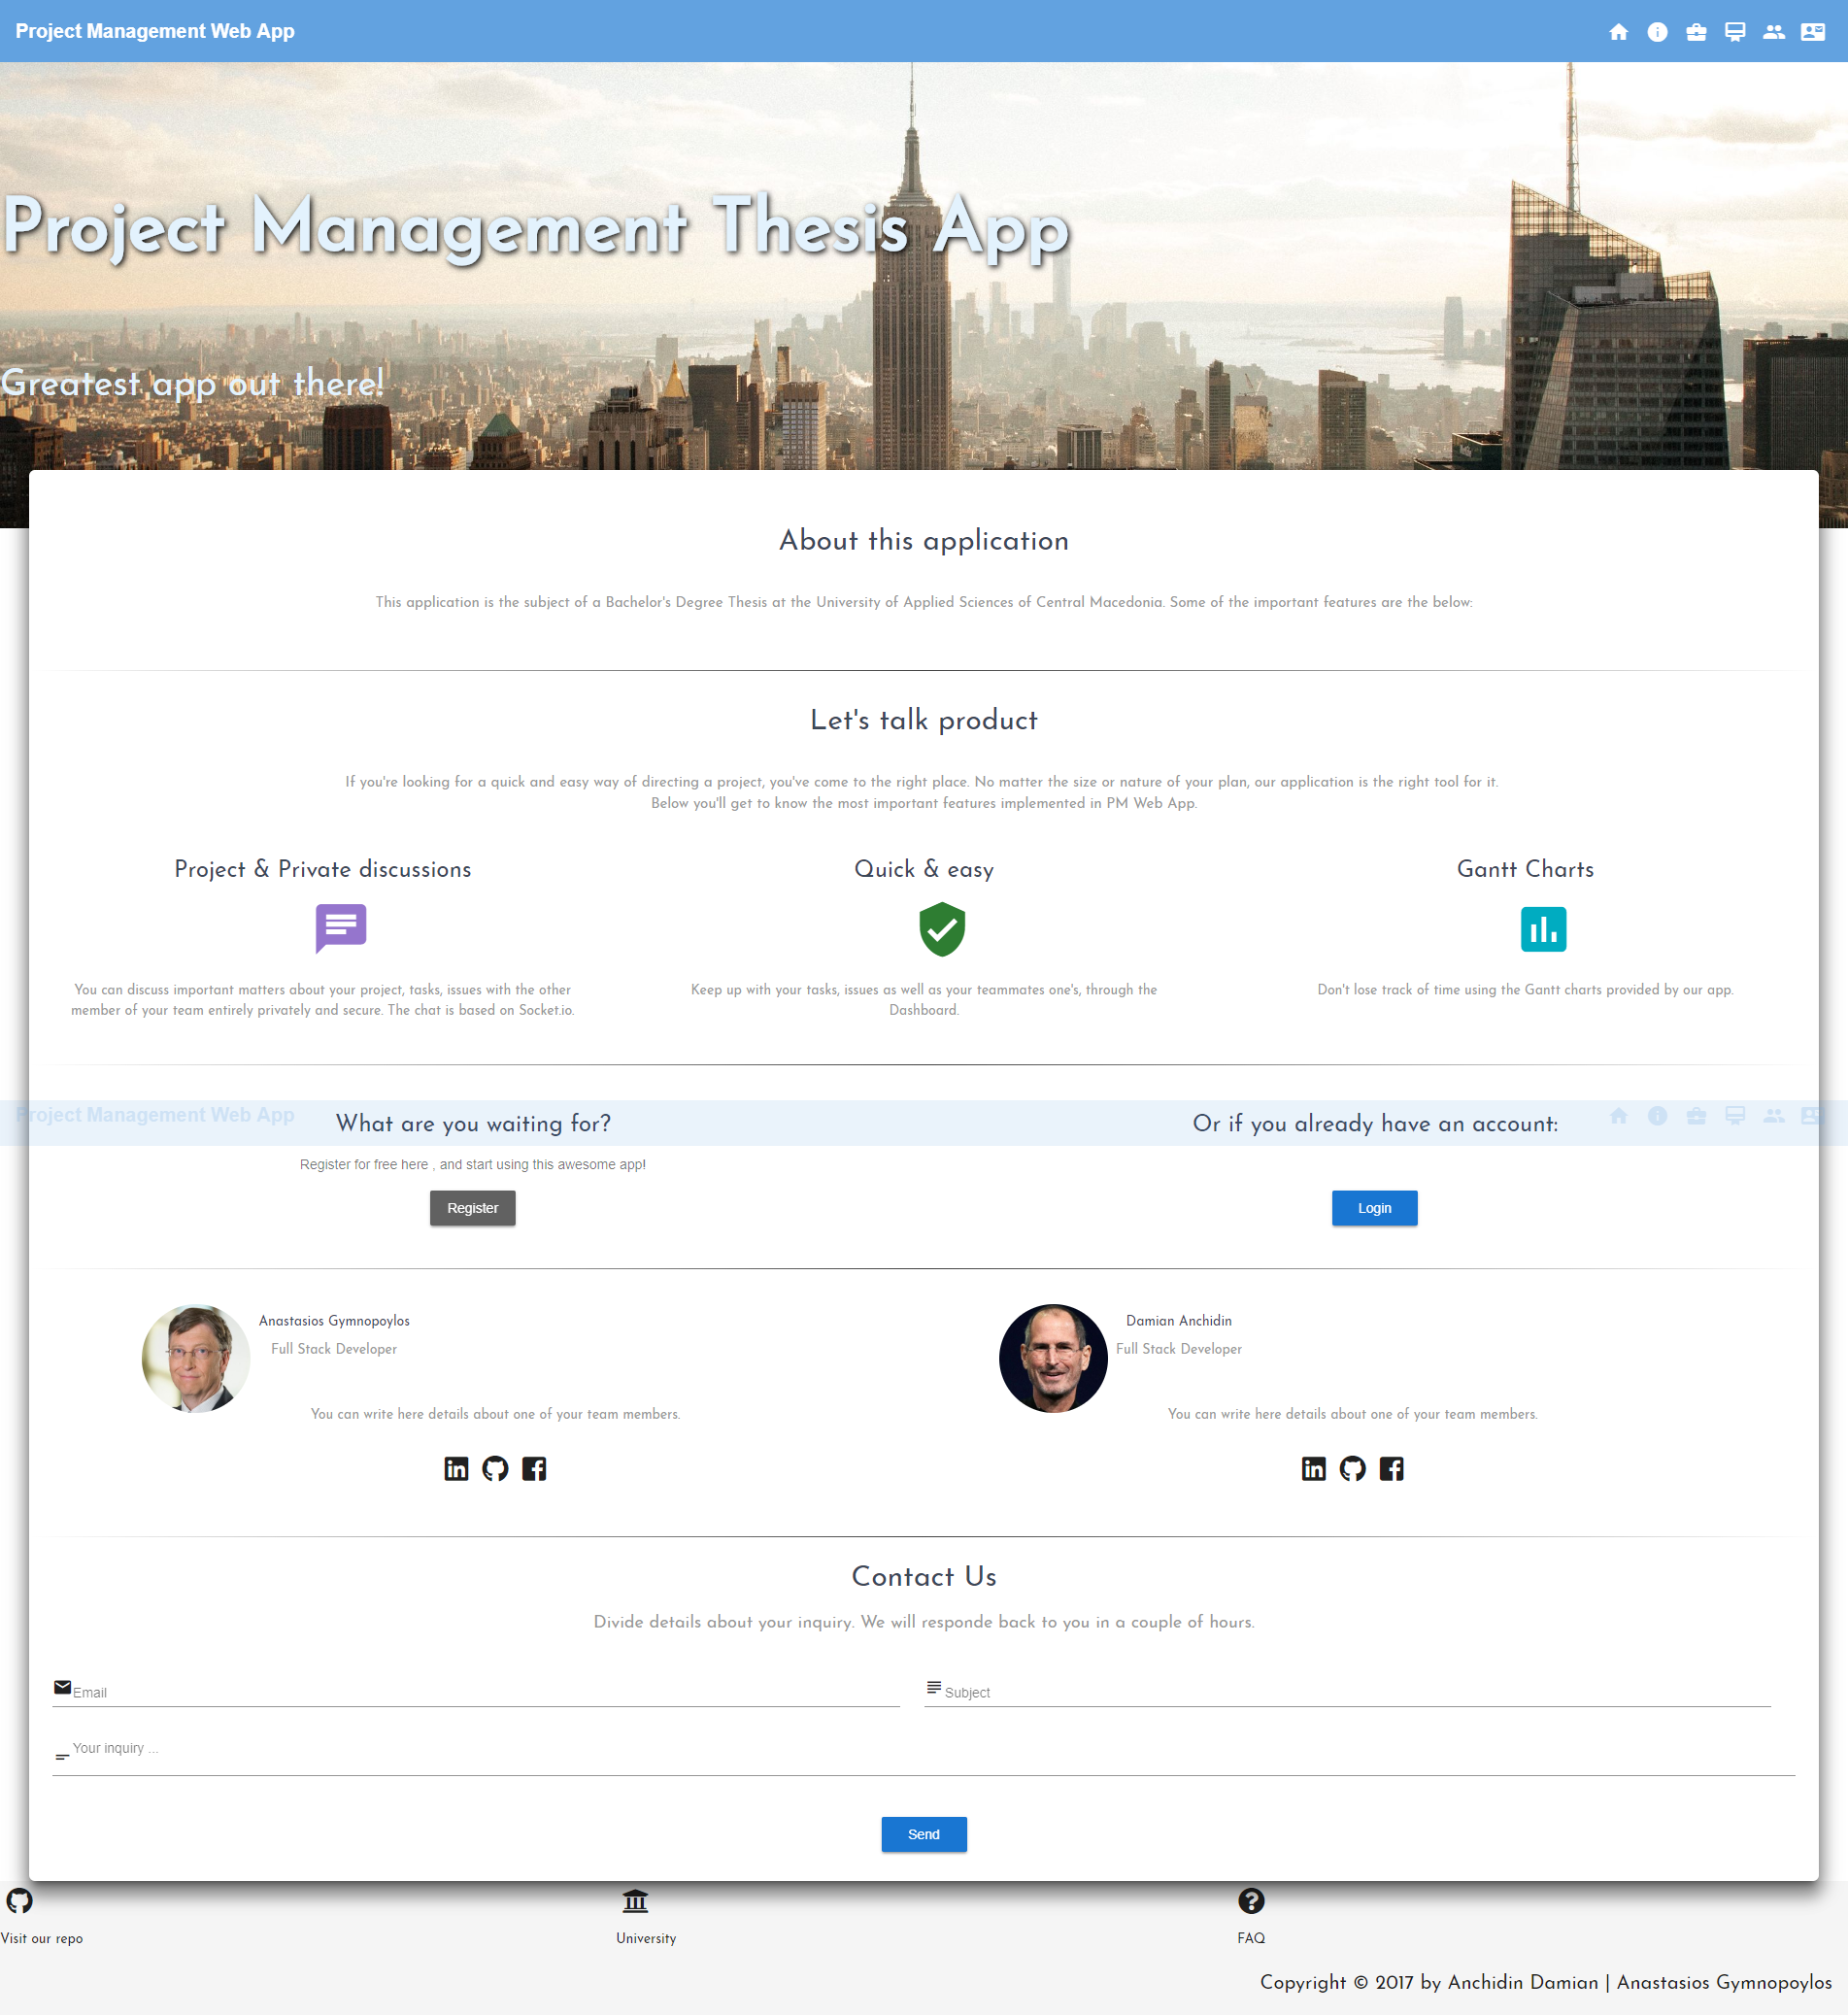
\includegraphics[scale=0.2]{images/homepage.png}
\caption{Αρχική σελίδα - \e{Homepage}}
\label{fig:homepage}
\end{figure}

\section{\e{Authentication}}
\pSpaceΉ εφαρμογή απαιτεί ένα λογαριασμό για να αποκτήσει ο χρήστης πρόσβαση στις υπηρεσίες που προσφέρονται.Ή εγγραφή αλλά και η είσοδος ολοκληρώνονται σε πολύ απλά βήματα.Προς το παρόν δεν υπάρχει δυνατότητα εγγραφής/ είσοδο με λογαρισμό κοινωνικού δικτύου.Αν ο χρήστης επιθυμεί να γυρίσει στην αρχική σελίδα, αυτό επιτυγχάνεται χρησιμοποιώντας την επιλογή του μένου που βρίσκεται στο πάνω μέρος της σελίδας. 

\subsection*{\e{Sign Up}}
\pSpaceΗ εγγραφή του χρήστη ακολουθεί μια βηματική μορφή για μια καλύτερη εμπειρία (βλ. σχ. \ref{fig:register}).\\
\pSpaceΤα βήματα πηγαίνουν ως εξής:\\
\begin{itemize}
	\item Αρχικά εμφανίζονται τρία πεδία για την ηλεκτρονική διεύθυνση, κωδικό και επαλήθευση κωδικού.Ο κώδικος πρέπει να έχει μήκος έξι χαρακτήρων και άνω, αλλιώς εμφανίζεται ένα σφάλμα που ενημερώνει τον χρήστη γι΄αυτήν την ιδιότητα.Επίσης υπάρχει δυνατότητα αποκάλυψης κωδικού για διευκολία.Ακόμη, σφάλματα σε περίπτωση που οι κωδικοί δεν είναι ίδιοι η αν η διεύθυνση δεν είναι έγκυρη εμφανίζονται σε πραγματικό χρόνο.Για να προχωρήσει στο επόμενο βήμα, δέν πρέπει να υπάρχουν σφάλματα ενεργά.
	\item Δύο ακόμη απαραίτητα πεδία υπάρχουν στο δεύτερο βήμα εγγραφής.Αφορούν το όνομα και το επίθετο του χρήστη.
	\item Στο τελευταίο βήμα, ο χρήστης έχει τρείς επιλογές: να γυρίσει στον προηγούμενο βήμα για να αλλάξει κάποιο πέδιο, \e{reset} φόρμας για να την ξανασυμπληρώσει και ολοκλήρωση διαδικασίας.
\end{itemize}
\pSpaceΑφού έχει ολοκληρωθεί με επιτυχία η εγγραφή του χρήστη, θα τον ανακατευθύνει στην σελίδα εισόδου.

\begin{figure}[!htb]
\centering
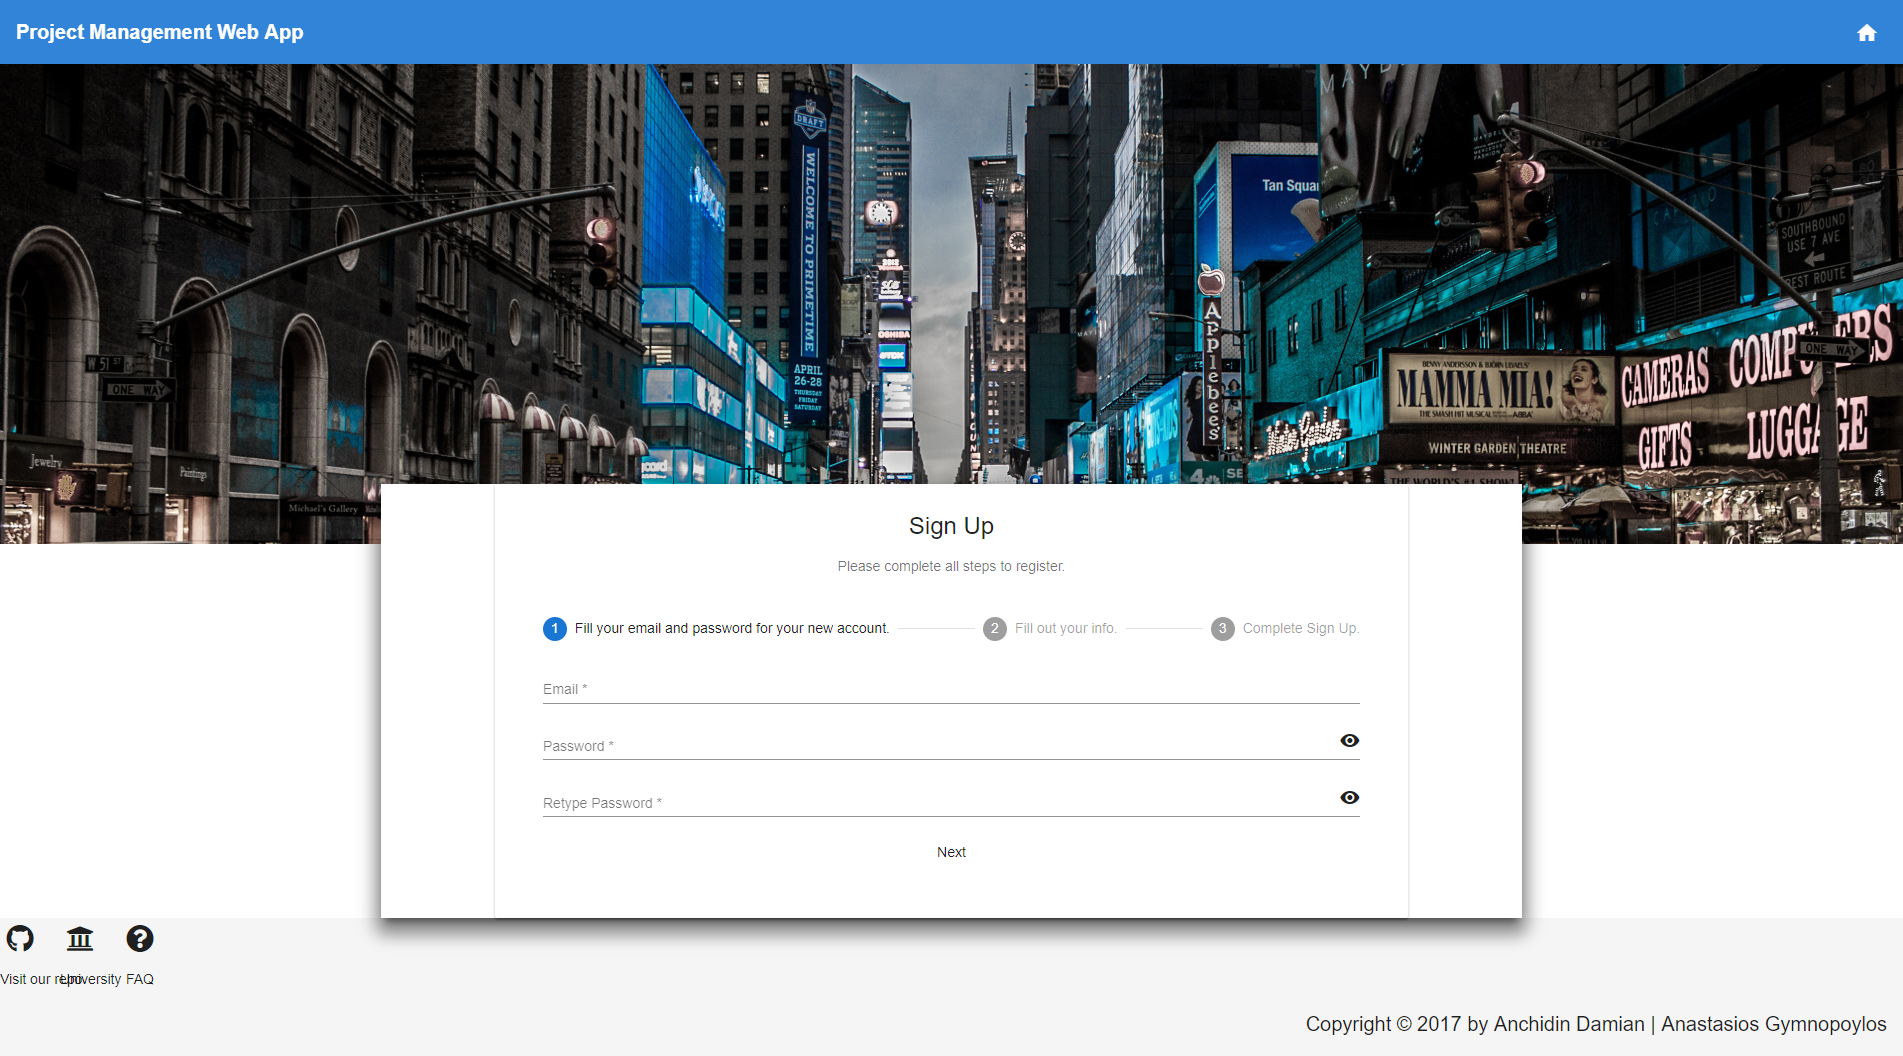
\includegraphics[scale=0.2]{images/register.png}
\caption{Εγγραφή - \e{Sign Up}}
\label{fig:register}
\end{figure}

\subsection*{\e{Sign In}}
\pSpaceΣυνηθίζεται για την είσοδο σε μια ηλεκτρονική υπηρεσία, να απαιτούνται μια ηλεκτρονική διεύθυνση και ένα κωδικό για επαλήθευση ταυτότητας.Τον ίδιο πρότυπο ακολυθείται και στην παρούσα εφαρμογή.\\
\pSpaceΟ χρήστης πληκτρολογεί το \e{email} και τον κωδικό, και σε περίπτωση απουσίας κάποιου σφάλματος, θα αποκτήσει πρόσβαση στις υπηρεσίες του \e{iPM}.Τα σφάλματα εμφανίζονται σε ένα \e{modal} παράθυρο με ένα μήνυμα που εξηγεί σε γενικές γραμμές το λάθος.Επίσης, όπως και στην εγγραφή, υπάρχει δυνατότητα αποκάλυψης κωδικού.Αν είναι επιτυχής η είσοδο, θα τον ανακατευθύνει στην εφαρμογή \e{iPM}.

\begin{figure}[!htb]
\centering
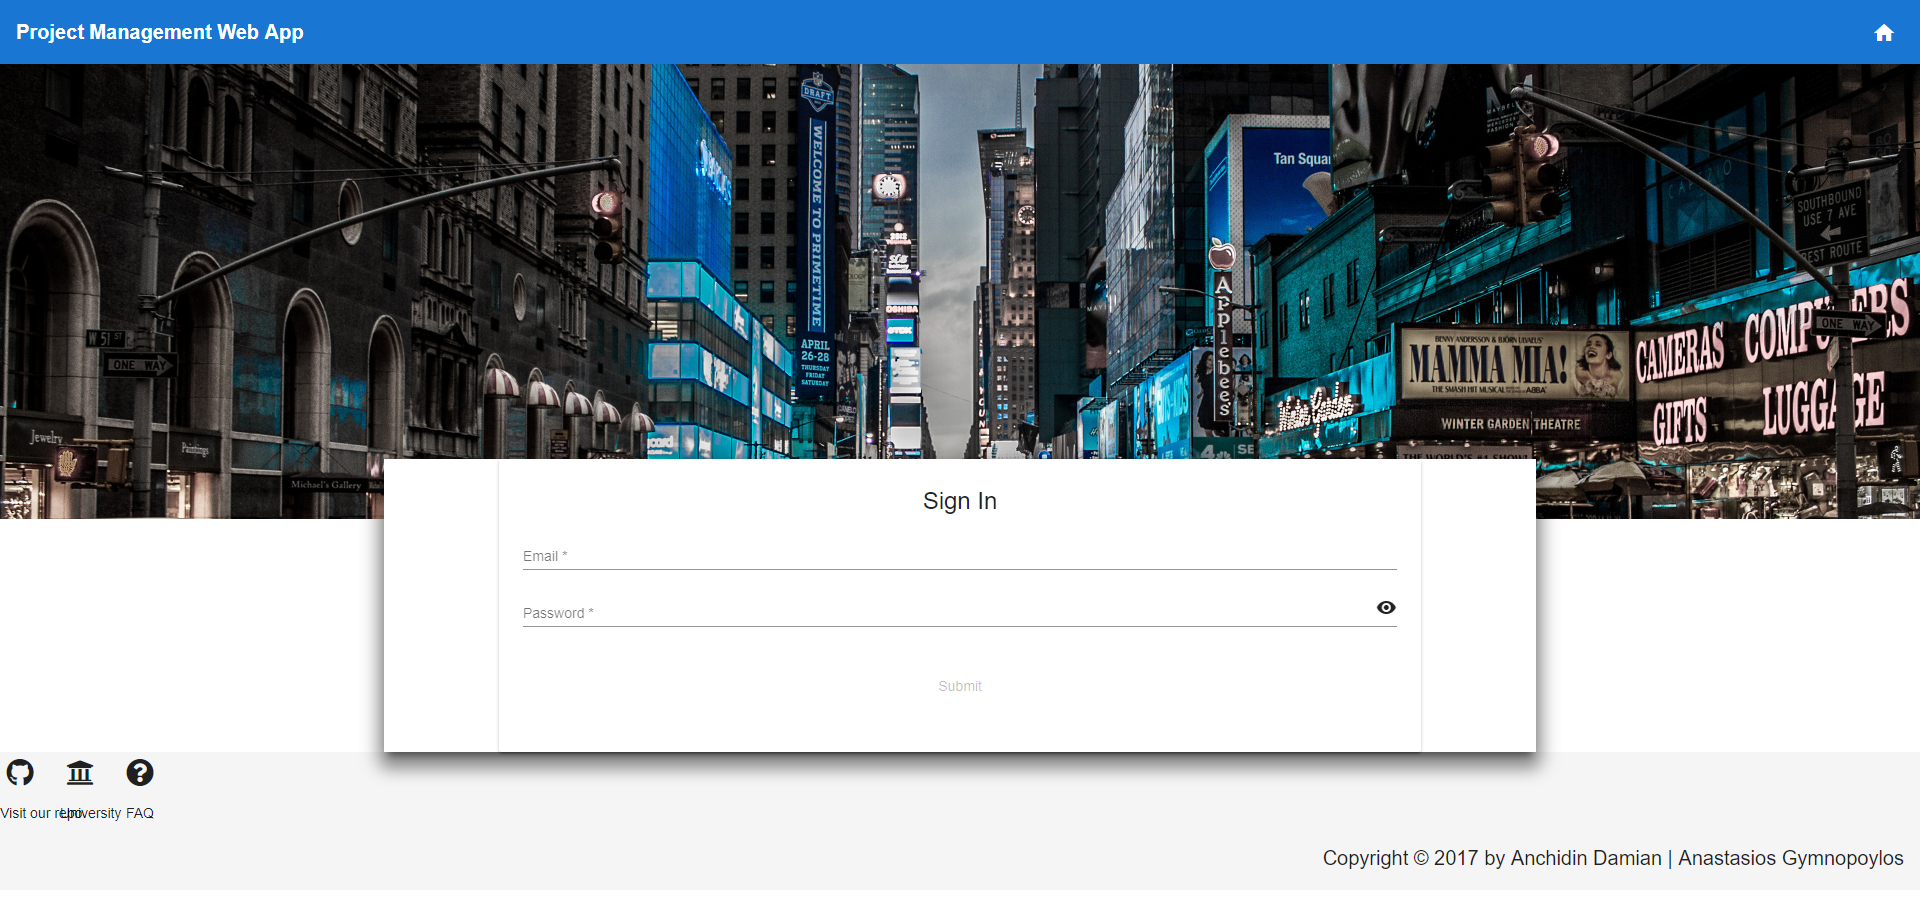
\includegraphics[scale=0.2]{images/login.png}
\caption{Είσοδο - \e{Sign In}}
\label{fig:login}
\end{figure}

\section{\e{iPM}}
\pSpaceΕφόσον έχει ολοκληρωθεί το στάδιο ταυτοποιήσης του χρήστη, θα αποκτήσει πρόσβαση στην διεύθυνση \e{\url{https://pmthesis.herokuapp.com/app}} όπου βρίσκεται η εφαρμογή \e{iPM}.Σημειώνεται πώς η εφαρμογή καταλαμβάνει αποθηκευτικό χώρο μέσω του \e{API} του περιηγητή, συγκεκριμένα το \e{Local Storage}.Αποθηκεύονται κάποιες ρυθμίσεις αλλά και το \e{token} που είναι απαραίτητο.Παρ'όλο που το \e{token} μπορεί να τον αποκωδικοποιήσει κανείς και να αλλάξει τις πληροφορίες του, μια τέτοια ενέργεια θα τον ακυρώσει με αποτέλεσμα να ανακατευθύνει τον χρήστη πάλι στην σελίδα εισόδου.Το ίδιο συμβαίνει και στην περίπτωση που λήγει η λείπει το παρόν \e{token}.\\
\pSpaceΗ σελίδα ακολουθεί τον ίδιο σχεδιασμό και στις δύο περιπτώσεις , χρήστη και έργο.Στο αριστερό μέρος υπάρχει το μενού με τις επιλογές που εξαρτώνται απο την ενότητα που βρίσκεται.Έχει την δυνατότητα απόκρυψης ώστε να μεγαλώσει ο χώρος δεδομένων.Στο επάνω μέρος, υπάρχουν κουμπιά που αφορούν τις ακόλουθες ενέργειες:\\
\begin{itemize}
	\item Το πρώτο στην σειρά είναι ένας διακόπτης για την απόκρυψη του αριστερού μενού.
	\item Δεύτερο είναι μια συντόμευση που επαναφέρει τον χρήστη στην αρχική σελίδα του \e{iPM}.
	\item Στην συνέχεια φαίνεται ένα πεδίο \e{Search} όπου ο χρήστης μπορεί να ψάξει έργα, άτομα και \e{task} για να διευκολυνθεί η διαχείριση έργων και εργασιών.
	\item Το επόμενο κουμπί εμφανίζει στο δεξίο μέρος της σελίδας τις ειδοποιήσεις.
	\item Ακολουθεί ένα κουμπί το όποιο ανοιγεί ένα μικρό \e{Context Menu} που περιέχει τέσσερις επιλογές για το θέμα σχεδιασμού.
	\item Τελευταίο είναι η αποσύνδεση, που ανακατευθύνει τον χρήστη στην σελίδα σύνδεσης.
\end{itemize}
\pSpaceΣτον υπόλοιπο χώρο φορτώνεται το δυναμικό περιεχόμενο.Θα αναφέρεται παρακάτω ως πλαίσιο δεδομένων.

% User actions
\subsection{\e{User}}
\pSpaceΑρχικά η εφαρμογή καλωσορίζει τον χρήστη, με τις ενέργειες που αφορούν τον ίδιο.Το μενού περιλαμβάνει τις ακόλουθες επιλογές, οι οποίες εξηγούνται σε λεπτομέρια παρακάτω:\\
\begin{itemize}
	\item \e{Dashboard}
	\item \e{My Projects}
	\item \e{My Tasks}
	\item \e{My Issues}
	\item \e{My Profile}
	\item \e{Calendar}
	\item \e{Chat}
	\item \e{Invites}
	\item \e{404}
\end{itemize} 

\subsubsection*{\e{Dashboard}}
\pSpaceΤο \e{Dashboard} βρίσκεται στην διεύθυνση \e{\url{http://pmthesis.herokuapp.com/app/dashboard}} και φορτώνει στον πλαίσιο δεδομένων, πέντε καρτέλες:
\begin{itemize}
	\item Η πρώτη είναι μια δοκιμστική καρτέλα, στην οποία ο χρήστης αλλάζει το μέγεθος καρτέλας.
	\item Η δεύτερη εμφανίζει τα \e{Tasks} που είναι αναθετημένα στον ίδιο, στις οποίες έχει περάσει ο χρόνος ολοκλήρωσης.Προς το παρόν δείχνει μόνο απλά \e{Tasks}.
	\item Η επόμενη καρτέλα προσφέρει συντομεύσεις για τα ενεργά έργα.
	\item Στην τέταρτη καρτέλα, περιέχονται τα πι πρόσφατα \e{Tasks} που αναθέτηκαν στον χρήστη.
	\item Η τελευταία καρτέλα έχει την ίδια λειτουργία με την προηγούμενη, αλλά για τα \e{Issues}.
\end{itemize}

\begin{figure}[!htb]
\centering
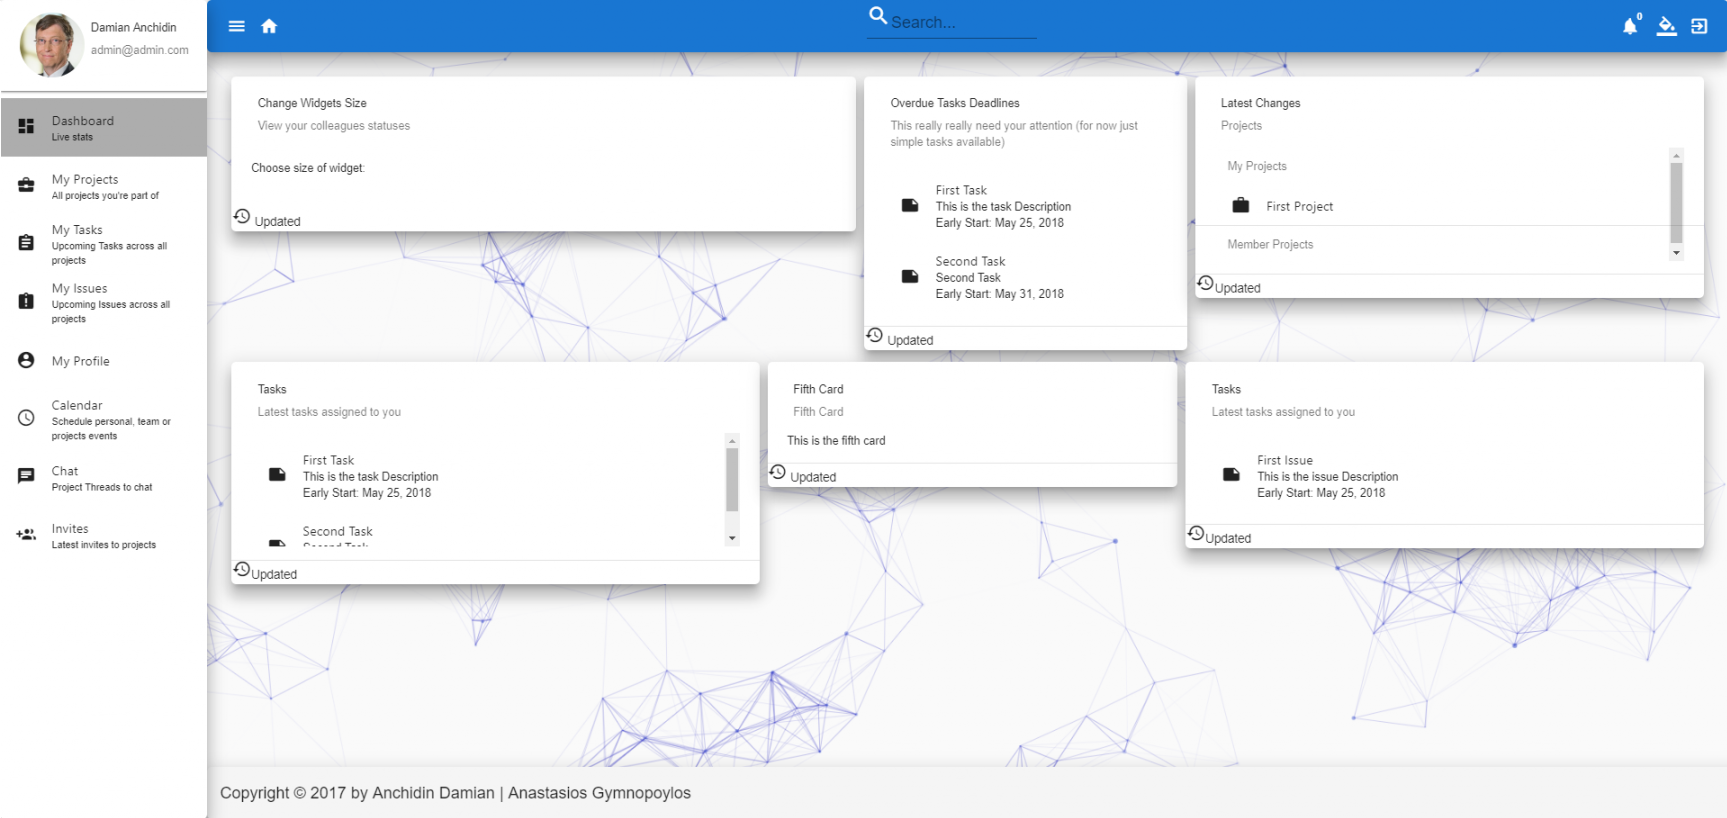
\includegraphics[scale=0.3]{images/userDashboard.png}
\caption{\e{User Dashboard}}
\label{fig:userDashboard}
\end{figure}

\subsubsection*{\e{My Projects}}

\subsubsection*{\e{My Tasks}}

\subsubsection*{\e{My Issues}}

\subsubsection*{\e{My Profile}}

\subsubsection*{\e{Calendar}}

\subsubsection*{\e{Chat}}

\subsubsection*{\e{Invites}}

\subsubsection*{\e{404}}
% /User actions

% Project actions
\subsection{\e{Project}}


\subsubsection*{\e{Dashboard}}

\subsubsection*{\e{Assignments}}

\subsubsection*{\e{Gantt}}

\subsubsection*{\e{Team}}

\subsubsection*{\e{Action Log}}

\subsubsection*{\e{Chat}}

\subsubsection*{\e{Settings}}
% /Project actions